\begin{document}
	
	\section{Pipeline Description}
	
	The aim of this work is to develop a pipeline which provides a good segmentation in a small amount of time; in order to achieve these aim, the pipeline must have the following characteristics:
	\begin{itemize}
		\item  \textbf{Fully Automated: } to remove the dependency from an external operator, and so the subjectivity of the segmentation; 
		
		\item \textbf{Fast: } in order to compete with certified software and to provides a segmentation in few minutes.
	\end{itemize}

	During the developing, the first problem we have to face was the lack of information: since COVID-19 is new disease, there aren't much data available. I've worked mainly on CT scans of 83 different patients provided by sant'Orsola hospital with manual segmentation, but also public dataset like MOSMED and ZENODO where used as benchmark. For each patient was available a manual segmentation, but even if some label seem to be of good quality and accurate, some other will present some errors and misclassified areas. In the end low number of patients and the quality of labels have discouraged us to use a supervised learning approach like classifiers or neural networks, an other reason is that a supervised approaches like Artificial Neural Network are computationally expansive and requires a lot of hardware resources and time.\\
	In the end a completely unsupervised technique was used, which doesn't requires to provides already segmented images as prior knowledge.\\
	An other thing to takes into account during the developing, is that the lesions may have different patterns according to the stage of the disease or the patients as in \figurename\,\ref{fig:GGO-Spatial} and usually these patterns are spatially disconnected, so to perform the segmentation a pixel classification techniques was used.
	
	\begin{figure}\label{fig:GGO-Spatial}
		\centering
		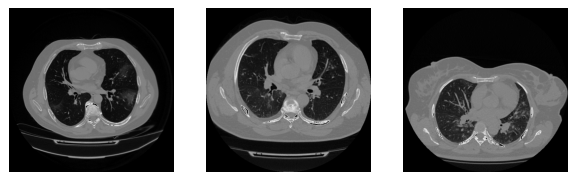
\includegraphics[scale=1.5]{GGOSeveralPatients.png}
		\caption{Groudf Glass Opacities of COVID-19 affected patients with different severity of the disease. From left to right this scans belong to CT-1, CT-2 and CT-4 category of MOSMED~\cite{DATA:MOSMED} dataset}
	\end{figure}
	
	In the end the basic idea was to use the Color Quantization as medical imaging segmentation , which aims to to identify the different type of tissue and lesions by grouping them by color similarity. In particular we aims to assign to each structure inside the lung a characteristic colors and label each voxel by identify it as belonging to the tissue with the most similar characteristic color. This approach is justified since exist a relation between the kind of tissue and the color used to display it in a CT scan, given by Hounsfield Unit.\\
	Since it is unlikely to find a structure with a single voxel extension, I've used the multi-channel characteristics of digital images to takes into accounts also the neighbouring voxels.\\
	
	In this section I will describe how color quantization works for image segmentation, how the color space was build in order to incorporate also neighbouring information and the final structure of the segmentation pipeline.
	
	
	 so we have to associate each pixel color to a particular tissue and, as we will see in the section below this will be done by using the Hounsfield Unit. In particular we will find the characteristic color of each lung tissue and assign each pixel to the tissue of the most similar characteristic color. 
	
	In this section I will discuss have applied the color quantization and I will describe the main structure of the developed pipeline.


\end{document}